\chapter{Elementary Logic}

\begin{chapqt}{Neil deGrasse Tyson}
I am convinced that the act of thinking logically cannot possibly be natural to the human mind. If it were, then mathematics would be everybody's easiest course at school and our species would not have taken several millennia to figure out the scientific method
\end{chapqt}

\begin{chapqt}{Robert Heinlein}
Anyone who cannot cope with mathematics is not fully human. At best he is a tolerable subhuman who has learned to wear shoes, bathe, and not make messes in the house.
\end{chapqt}

\section*{Introduction}

In some sense, this text is about mathematical proofs. Why do mathematicians require proofs? How are you supposed to read and understand a proof?  If you have to prove something yourself, how do you know where to start?  How do you know when you're finished? Perhaps most importantly, what is a proof?

Mathematicians use proofs for many reasons, but a very simple answer to the last question above is that a proof is a logical argument to show that a statement is true.  Unlike the experimental sciences, mathematicians do not accept a statement as true based on data or on statistical reasoning.  We might collect data, but only to determine whether or not we believe that something is true.  Consider the following:

\medbreak\noindent
{\bf Theorem.} \emph{If $p$ is an even integer, then $p^2$ is even.}
\medbreak

This statement is true, but how do we know that?  We may start by squaring some even integers: $2^2=4$ is even, $8^2=64$ is even, $(-12)^2=144$ is even. Try a few more on your own. While this kind of experimentation certainly leads us to believe the statement is true, how can we be sure the pattern we think we see is always true? A statement like this one claims that something is true for \emph{all} even integers. There are infinitely many even integers, so we can't possibly try all of them! However unlikely it may seem, it is possible that the first 3,000,012 examples we try will work, but the next one won't, or even that the statement is true for all but a single even integer.\footnote{If this seems impossible, consider the following statement: \emph{Every prime number is odd.}} In order to be certain that such a statement is true, we must carefully define what it means for an integer to be even, then use that property to prove that the square of \emph{every} even integer is even. We will return to this example in the next chapter.

\section{Propositions}

\begin{definition}
A \emph{proposition}\index{proposition|textbf} is a statement that is either true or false, but not both.  The \emph{truth value} \index{truth value|textbf} of a proposition is true (T) if the sentence is true and false (F) if the sentence is false.
\end{definition}

 Let's consider several sentences.

\begin{itemize}\itemsep0pt
\item \emph{Two plus two equals four.} This sentence is true, hence a proposition.
\item \emph{Seven minus three equals twelve.} This sentence is false, hence a proposition. 
\item \emph{It will snow in Grand Forks on March 17, 2525.} This sentence is either true or false, even if nobody currently alive will ever know which. It is a proposition, we just don't happen to know the truth value.
\item \emph{Go clean your room.} This sentence is a command, not a proposition.
\item \emph{Is it raining outside?} Again, this is not a proposition. It is a question.
\item \emph{This sentence is false.} This sentence is not a proposition because it cannot be either true or false. If it is true, then it's claim is false. If it's false, then it's claim must be true. We will not allow sentences that refer to themselves except as examples of what might go wrong if we are not careful.
\item \emph{$x+3=12$.} This sentence cannot be said to be true or false without more information about the variable $x$. If $x=0$, then it is false. If $x=9$, then it is true. Statements like this are not propositions, but are extremely important. We will discuss them in detail in Section [\ref{PredQuant}].
\end{itemize}

We will use uppercase letters, frequently $P$ or $Q$, to stand for variable propositions in much the same way that you might use $x$ or $y$ to represent variable numbers in algebra.

\section{Connectives and Truth Tables}

Many of the propositions we are interested in are made up of more elementary propositions. For example, the proposition $S$: \emph{today is Tuesday and it's raining} is made up of the two propositions $P$: \emph{today is Tuesday} and $Q$: \emph{it's raining}. The word \emph{and} in $S$ is called a connective \index{connective} since it gives us a way to connect two propositions and form another.  In this section we will look at several kinds of connectives, beginning with conjunction.

\subsection{Conjunction} 

\begin{definition}
The \emph{conjunction} \index{connective!conjunction|textbf} of the propositions $P$ and $Q$ is the proposition \emph{$P$ and $Q$}, denoted $P\land Q$. The conjunction $P\land Q$ is true when both $P$ and $Q$ are true and false if either $P$ or $Q$ (or both) are false. 
\end{definition}

We will sometimes keep track of the truth values \index{truth value} of propositions in a \emph{truth table} \index{truth table|textbf}, where we list the truth values of a propositions in terms of the truth values of elementary propositions.

\begin{center}
\begin{tabular}[t]{|c|c|c|}
\hline
$P$ & $Q$ & $P\land Q$ \\
\hline
\hline
T & T & T \\
\hline
T & F & F \\
\hline
F & T & F \\
\hline
F & F & F \\
\hline
\end{tabular}
\end{center}

The table above indicates that when $P$ and $Q$ are both true, $P\land Q$ is true; when $P$ is true and $Q$ is false, $P\land Q$ is false; etc. Note that in this case there are four rows in the table. For a proposition made up of $n$ elementary propositions, there will be $2^n$ rows in the truth table\index{truth table} because there are two possible truth values for each of the elementary propositions. This makes it cumbersome to construct truth tables for very complicated propositions. Nevertheless, we will find them to be a convenient tool.

\subsection{Disjunction}

We next consider propositions of the form \emph{$P$ or $Q$}. We have to be a bit more careful defining what we mean in this case, because the word \emph{or} can be ambiguous in english. Let's consider a couple of english sentences to see why:

\begin{itemize}
\item \emph{Either it's Tuesday or it's raining.} 
\item \emph{Do you prefer coffee or tea?}
\end{itemize}

In the first of these sentences we mean that at least one of the two conditions must be met, it's Tuesday or it's raining. If it's raining on a Tuesday, this proposition is still true. In this case \emph{or} is inclusive in the sense that it includes the possiblity that both conditions are met. In the second sentence, we presume that only one of the two options is possible.
This use of the word \emph{or} is exclusive since it excludes the possibility of both conditions being true at the same time. In normal discourse this kind of ambiguity doesn't usually cause any difficulty because we can determine the meaning from the context. We do not want to allow this kind of ambiguity in logical propositions, so we always use the word \emph{or} in the inclusive sense. In other words, $P\lor Q$ is true if at least one of $P$ or $Q$ is true. 

\begin{definition}
The \emph{disjunction}\index{connective!disjunction|textbf} of $P$ and $Q$ is the proposition \emph{$P$ or $Q$}, denoted $P\lor Q$, which is true whenever at least one of $P$ or $Q$ is true.
\end{definition}

Here is a truth table for the proposition $P\lor Q$.

\begin{center}
\begin{tabular}[t]{|c|c|c|}
\hline
$P$ & $Q$ & $P\lor Q$ \\
\hline
\hline
T & T & T \\
\hline
T & F & T \\
\hline
F & T & T \\
\hline
F & F & F \\
\hline
\end{tabular}
\end{center}

\subsection{Implication} 

Most mathematical propositions have the form \emph{If $P$, then $Q$}. Of course, either of $P$ or $Q$ might be propositions made of several other propositions.  \index{connective!implication|see{implication}}

Let's consider an example:
\smallbreak\noindent
\emph{If the student is on the basketball team, then she won't be in class on Friday.}
\smallbreak\noindent
Consider two students in my Friday class, Jill and Pat. We will assume that Jill is on the basketball team and that Pat is not. Most of us would agree that Jill will not be in class Friday if the statement is true, so if Jill is in class then the statement must be false. What does the statement tell us about Pat? If she shows up for class Friday there's certainly nothing false about the statement, but what if she doesn't show up for class? Does that make the statement false? No! The statement makes no claim about Pat, so her attendence or absence doesn't impact the truth of the statement. 

\begin{definition}
The proposition \emph{If $P$, then $Q$} is called an \emph{implication} \index{implication|textbf} and is denoted $P\Rightarrow Q$. The proposition $P$ is the \emph{hypothesis} \index{implication!hypothesis} of the implication and $Q$ is the \emph{conclusion}.\index{implication!conclusion} The implication is false only when $P$ is true and $Q$ is false.
\end{definition}

Here is a truth table for $P\Rightarrow Q$.

\begin{center}
\begin{tabular}[t]{|c|c|c|}
\hline
$P$ & $Q$ & $P\Rightarrow Q$ \\
\hline
\hline
T & T & T \\
\hline
T & F & F \\
\hline
F & T & T\\
\hline
F & F & T\\
\hline
\end{tabular}
\end{center}

\medbreak
As a student of mathematics, it is absolutely essential that you understand what an implication means and what it doesn't mean.  To say that $P\Rightarrow Q$ is true does not mean that $P$ is true or that $Q$ is true, it does mean that there is a relationship between the truth values of these two propositions.  The implication $P\Rightarrow Q$ is false when $P$ is true and $Q$ is false; it is true when either $P$ is false or $Q$ is true. 

There are several related implications related to the implication $P\Rightarrow Q$ that we will occassionally find these useful. Be aware that these are not all equivalent. You will determine which are equivalent to the original implication in Exercise \ref{exer:contrapos}.
\begin{definition} 
For the implication $P\Rightarrow Q$:
\begin{itemize}\itemsep0pt
\item The \emph{converse}\index{implication!converse|textbf}  is $Q\Rightarrow P$.
\item The \emph{contrapositive}\index{implication!contrapositive|textbf}  is $\neg Q\Rightarrow\neg P$.
\item The \emph{inverse}\index{implication!inverse|textbf} of is $\neg P\Rightarrow\neg Q$.
\end{itemize}
\end{definition}

\subsection{Logical Equivalence}

\begin{definition}
Two propositions $P$ and $Q$ are said to be \emph{logically equivalent} \index{logical equivalence|textbf} if they always have the same truth value. We use the connective \emph{iff}, read ``if and only if,'' and use the symbol $\Leftrightarrow$. The proposition $P\Leftrightarrow Q$ is true when $P$ and $Q$ have the same truth value. 
\end{definition}

\begin{center}
\begin{tabular}[t]{|c|c|c|}
\hline
$P$ & $Q$ & $P\Leftrightarrow Q$ \\
\hline
\hline
T & T & T \\
\hline
T & F & F \\
\hline
F & T & F\\
\hline
F & F & T\\
\hline
\end{tabular}
\end{center}

\subsection{Negation}\label{neg1}

\begin{definition}
The \emph{negation}\index{negation|textbf} of $P$, denoted $\neg P$ and sometimes read ``not $P$,'' is the proposition whose truth value is always opposite that of $P$. 
\end{definition}

Note that negation is not actually a connective since it applies to a single proposition rather than connecting two propositions.

\begin{center}
\begin{tabular}[t]{|c|c|}
\hline
$P$ & $\neg P$\\
\hline
\hline
T & F\\
\hline
F & T\\
\hline
\end{tabular}
\end{center}

\subsection{Tautology and Contradiction}

\begin{definition}
A \emph{tautology}\index{tautology|textbf} is a proposition that is always true, regardless of the truth values of the elementary propositions that make it up.
\end{definition}

\begin{definition} 
A \emph{contradiction}\index{contradiction|textbf} is a proposition that is always false.
\end{definition}

\begin{example}
The proposition $P\lor \neg P$ is an example of a tautology.  One way to see this is to look at a truth table.  Notice that all truth values in the column for $P\lor \neg P$ are true.  We can also use this truth table to see that $P\land\neg P$ is a contradiction because every truth value in that column is false.

\begin{center}
\begin{tabular}[t]{|c|c|c|c|}
\hline
$P$ & $\neg P$ & $P\lor \neg P$ & $P\land \neg P$\\
\hline
\hline
T & F & T & F\\
\hline
F & T & T & F\\
\hline
\end{tabular}
\end{center}
\end{example}

\begin{example}
Use truth tables to show that the following are tautologies.
\begin{enumerate}\itemsep0pt
\item $P\Rightarrow(P\lor Q)$
\item $(P\Rightarrow Q)\Leftrightarrow(\neg Q\Rightarrow \neg P)$
\end{enumerate}
{\bfseries\upshape Solutions}
\begin{enumerate}\itemsep0pt
\item We must construct a truth table with a column for $P\Rightarrow(P\lor Q)$ and show that the truth values in that column are all T.
\begin{center}
\begin{tabular}[t]{|c|c|c|c|}
\hline
$P$ & $Q$ & $P\lor Q$ & $P\Rightarrow(P\lor Q)$ \\
\hline
\hline
T & T & T & T \\
\hline
T & F & T & T \\
\hline
F & T & T & T \\
\hline
F & F & F & T \\
\hline
\end{tabular}
\end{center}
\item Note that we can either construct a truth table with a column for the desired equivalence and show that the truth values are all T, or we can construct a truth table with the columns for $P\Rightarrow Q$ and $\neg Q\Rightarrow \neg P$ and show that the truth values are always equal to each other. We will do the latter since it is less work.
\begin{center}
\begin{tabular}[t]{|c|c|c|c|c|c|}
\hline
$P$ & $Q$ & $\neg P$ & $\neg Q$ & $P\Rightarrow Q$ & $\neg Q\Rightarrow \neg P$ \\  
\hline
\hline
T & T & F & F & T & T \\ 
\hline
T & F & F & T & F & F \\
\hline
F & T & T & F & T & T \\
\hline
F & F & T & T & T & T \\
\hline
\end{tabular}
\end{center}
\end{enumerate}
\end{example}

\section{Predicates, Instantiation, and Quantification}\label{PredQuant}

We return our attention now to statements that involve variables, like $x+3=12$. Such a statement is called a \emph{predicate}\index{predicate|textbf} and we will usually indicate it with $P(x)$ rather than $P$. Before a predicate takes on a truth value, we need to know something about the variable. We noted before that if $x=0$, then the statement is false; but if $x=9$, then the statement is true. What if $x$ represents my desk? In that case the statement is complete nonsense, but you probably feel like there's something a little bit unfair about that choice for $x$. We see an equation and usually think that the variable must represent a number, right? The first thing you should know about any variable in a predicate is what it can represent. This is called the \emph{universe}\index{universe|textbf} or the \emph{domain of discourse}. \index{domain of discourse|see {universe}} In mathematics, we will be very explicit about what universe we are talking about.

\subsection{Instantiation}

Let's understand that in our predicate $P(x)$ from the previous paragraph, we declare that the universe is the set of real numbers. That still doesn't turn $P(x)$ into a proposition because, as noted above, $P(x)$ doesn't take on a truth value until we know which real number $x$ indicates. One way to do this is called \emph{instantiation}, \index{instantiation|textbf} which means choosing a particular value for the variable(s). Consider for example the sentence: \emph{Let $x=2$, then $x+3=12$.} In this case the sentence is a proposition with truth value F.

The other option is \emph{quantification}\index{quantifier} of the variable(s). We will discuss two kinds of quantifiers, \emph{universal} and \emph{existential}.  You might occasionally encounter other quantifiers, but they are not necessary. 

\subsection{Universal Quantification}

\begin{definition}
A \emph{universal quantifier}\index{quantifier!universal|textbf} indicates that the predicate is true for all instances of the variable in the given universe.  It is typically indicated by using the phrase ``for every'' or ``for all,'' and can be denoted symbolically by $\forall$ in symbolic statements. 
\end{definition}

The following sentences are universally quantified propositions. Only the second is true. 

\begin{itemize}\itemsep0pt
\item \emph{For every real number $x$, $x+3=12$.}
\item \emph{The square of $x$ is nonnegative for all real $x$.}
\item \emph{The square of $x$ is nonnegative for all complex $x$.}
\end{itemize}

\subsection{Existential Quantification}
 
\begin{definition}
An \emph{existential quantifier}\index{quantifier!existential|textbf} indicates that the predicate is true for at least one instance of the variable in the given universe.  It is typically indicate by the phrase ``for some'' or ``there exists,'' and can be denoted by $\exists$ in symbolic statements. 
\end{definition}

The following sentences are existentially quantified. All three of these are true.

\begin{itemize}\itemsep0pt
\item \emph{There is a real number $x$ so that $x+3=12$.}
\item \emph{The square of $x$ is nonnegative for some real $x$.}
\item \emph{The square of $x$ is nonnegative for some complex $x$.}
\end{itemize}

\subsection{Syllogisms and Venn Diagrams}

A \emph{syllogism}\index{syllogism} is a form of logical argument that deduces a conclusion based on two premises. For example:

\begin{center}
{\slshape All men are mortal. Socrates is a man. Hence Socrates is mortal.}
\end{center}

This is a valid syllogism. If we assume that the premises are true, then the conclusion must follow. One tool we can use to help think about syllogisms is a \emph{Venn diagram},\index{Venn diagram|textbf} which in it's simplest form is a collection of circles that represent the various categories in the premises. In this case we will have one circle representing mortals and another representing men. Since one of our premises is that all men are mortal, the circle representing men is completely contained inside the circle representing mortals:

\vennAll{mortal}{men}

Since Socrates is a man, hence inside the circle representing men, he must of necessity also be inside the circle representing mortals, hence the syllogism is valid. 

\begin{example}
Determine whether each of the following syllogisms is valid.
\begin{enumerate}\itemsep0pt
\item Some students are freshmen. Pat is a student. Hence Pat is a freshman.
\item No cats are dogs. Jade is a cat. Hence Jade is not a dog.
\item Some cats are psychopaths. Jawa is a cat. Hence Jawa is a psychopath.
\item Some Billywiggles are Bleepzigs. Some Bleepzigs are Jabberwoks. Hence some Billywiggles are Joabberwoks.
\end{enumerate}
{\upshape\bfseries Solutions}
\begin{enumerate}\itemsep0pt
\item The circle for students should overlap the circle for freshmen, but need not be contained within it since our assumption is that only some students are freshmen.. Here is a \index{Venn diagram|(} Venn diagram:
\vennSome{freshmen}{students}
Note that Pat may be in the student circle without being inside the freshmen circle, so the syllogism is not valid. 
\item In this case, the circle for cats should be completely outside the circle for dogs since no cats are dogs. Here is a Venn diagram:
\vennNone{dogs}{cats}
Since Jade must be within the cats circle, Jade cannot be within the dogs circle, so the syllogism is valid.
\item Here is a Venn diagram:
\vennSome{psychopaths}{cats}
Since Jawa must be in the cats circle, but may or may not be within the psychopaths circle, this syllogism is not valid.
\item This requires a slightly more complicated Venn diagram, and we must be very careful about what is absolutely necessary. It is possible for the Venn diagram to look like this:
\begin{center}
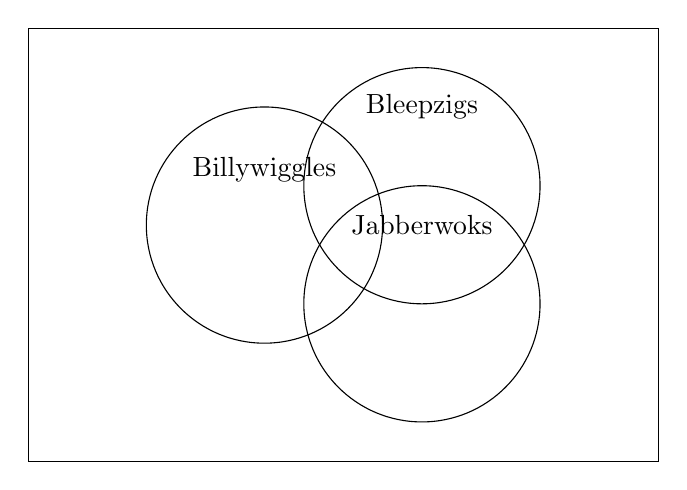
\begin{tikzpicture}
\draw (-4,-3) -- (4,-3) -- (4,2.5) -- (-4,2.5) -- cycle;
\draw (1,.5) circle [radius=1.5] (1,1.5) node {Bleepzigs};
\draw (-1,0) circle [radius=1.5] (-1,.7) node {Billywiggles};
\draw (1,-1) circle [radius=1.5] (1,0) node {Jabberwoks};
\end{tikzpicture}
\end{center}
On the other hand, it is also possible for the Venn diagram to look like the following:
\begin{center}
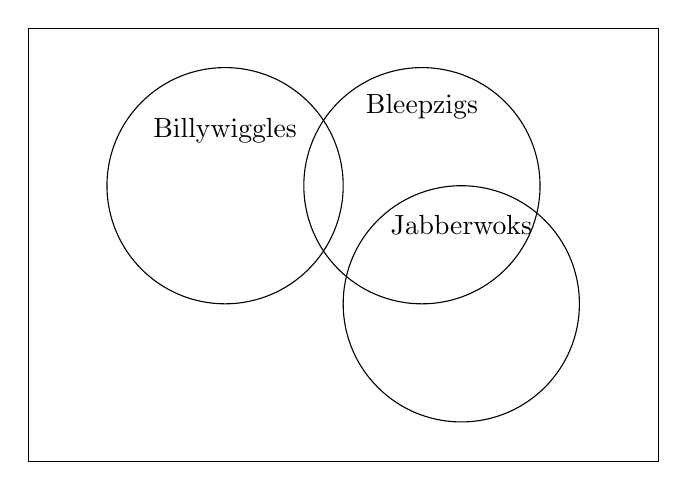
\begin{tikzpicture}
\draw (-4,-3) -- (4,-3) -- (4,2.5) -- (-4,2.5) -- cycle;
\draw (1,.5) circle [radius=1.5] (1,1.5) node {Bleepzigs};
\draw (-1.5,.5) circle [radius=1.5] (-1.5,1.2) node {Billywiggles};
\draw (1.5,-1) circle [radius=1.5] (1.5,0) node {Jabberwoks};
\end{tikzpicture}
\end{center}
This syllogism is not valid.\index{Venn diagram|)}
\end{enumerate}
\end{example}

\subsection{Quantification of Several Variables}

A predicate can have two or more variables. In order to use the predicate in a proposition, a universe\index{universe} must be declared for each variable and each variable must be instantiated or quantified. We will discuss the various ways a two variable predicate might be quantified by considering an example.

We consider the predicate $P(x,y)$ given by $x+y=0$. Throughout, we will will assume that the universe for both $x$ and $y$ is the set of real numbers.\footnote{In general, distinct variables might sometimes come from different universes.} Without redefining the universe every time, both variables could be universally quantified,\index{quantifier!universal} both could be existentially quantified,\index{quantifier!existential} or one could be universally quantified and the other existentially quantified. We are particularly interested in determining when each proposition will be true and whether the order of the quantifiers matters.

\begin{itemize}\itemsep0pt
\item $\forall x\ \forall y\ P(x,y)$: This proposition can be read as \emph{for all (real) $x$ and for all (real) $y$, $x+y=0$}, which says the sum of any two real numbers is 0. Clearly this is false. 
\item $\forall y\ \forall x\ P(x,y)$: Restating this as we did above, it is not difficult to see that this proposition is equivalent to the first one.
\item $\exists x\ \exists y\ P(x,y)$: We can read this as \emph{there is an $x$ so that there is a $y$ so that $x+y=0$}, which says that there are real numbers $x$ and $y$ such that $x+y=0$. This is true. Once again, reversing the order of the quantifiers doesn't matter.
\item $\forall x\ \exists y\ P(x,y)$: This proposition says that \emph{for every $x$ there is a $y$ such that $x+y=0$}, in other words every real number has an additive inverse, which is certainly true.
\item $\exists y\ \forall x\ P(x,y)$: The variables here are quantified the same, but the order is changed. Does that matter? The proposition this time says \emph{there is a $y$ so that for all $x$, $x+y=0$}. In other words, there is some real number $y$ so that adding any real number to $y$ yields a sum of 0, which is certainly false!
\end{itemize}

The moral of the last example is that you must be careful to quantify variables in the correct order when some variables are universally quantified and some are existentially quantified.

\section{Negations}

As mentioned previously in [\ref{neg1}], the negation of a proposition\index{negation} is the proposition with the opposite set of truth values.  In this section we are going to discuss the negations of compound propositions, which can be an important step in some kinds of proofs. We begin with two theorems that tell how to find the negations of propositions involving connectives.

\begin{thrm}\label{thrm:negimp}
Given any propositions $P$ and $Q$, $\neg(P\Rightarrow Q)\Leftrightarrow (P\land\neg Q)$.
\end{thrm}

To see that this theorem is true, we first make sure that we understand what it is saying. The variables in this case are actually propositions $P$ and $Q$, both of which are universally quantified. The theorem asserts that the compound proposition $\neg(P\Rightarrow Q)\Leftrightarrow (P\land\neg Q)$ is always true, so we must demonstrate that no matter what the truth values of $P$ and $Q$ are, the statement in the theorem is a tautology. We proceed by constructing a truth table.

\begin{center}
\begin{tabular}[t]{|c|c|c|c|c|c|}
\hline
$P$ & $Q$ & $\neg Q$ & $P\Rightarrow Q$ & $ \neg(P\Rightarrow Q)$ & $P\land \neg Q$ \\
\hline
T & T & F & T & F & F \\
\hline
T & F & T & F & T & T \\
\hline
F & T & F & T & F & F \\
\hline
F & F & T & T & F & F \\
\hline
\end{tabular}
\end{center}

The truth of the next theorem can be established in a similar fashion, which we leave tothe exercises (see  \ref{exer:DeMorgan}). 

\begin{thrm}\label{thrm:DeM}
{\bfseries\upshape (DeMorgan's Laws)} \index{DeMorgan's Laws|textbf}
Given any propostions $P$ and $Q$:
\begin{enumerate}
\item $\neg (P\land Q)\Leftrightarrow (\neg P\lor\neg Q)$
\item $\neg (P\lor Q)\Leftrightarrow (\neg P\land\neg Q)$
\end{enumerate}
\end{thrm}

We can use these results to understand the negations of more complicated propositions. Suppose we want to know how to negate the proposition $P\Rightarrow(Q\land R)$. We apply what we know one step at a time, beginning with the implication:
\begin{equation*}
\begin{split}
\neg \bigl(  P\Rightarrow (Q\land R)\bigr) &\Leftrightarrow P\land\bigl( \neg(Q\land R)\bigr) \qquad\text{ (Theorem \ref{thrm:negimp})}\\
&\Leftrightarrow P\land (\neg Q \lor \neg R) \qquad\text{ (Theorem \ref{thrm:DeM}(i))}\\
\end{split}
\end{equation*}

\begin{example}
Find the negation of each of the following propositions.
\begin{enumerate}\itemsep0pt
\item $P\land(Q\Rightarrow R)$
\item $(P\lor Q) \land (P\lor R)$
\end{enumerate}
{\bfseries\upshape Solutions}
\begin{enumerate}\itemsep0pt
\item We apply Theorems \ref{thrm:negimp} and \ref{thrm:DeM} where indicated.
\begin{equation*}\begin{split}
\neg\bigl( P\land (Q\Rightarrow R)\bigr) &\Leftrightarrow \bigl(\neg P \lor \neg(Q\Rightarrow R)\bigr) \qquad \text{(Theorem \ref{thrm:DeM}(i))}\\
&\Leftrightarrow\bigl( \neg P \lor(Q\land\neg R) \bigr) \qquad\text{(Theorem \ref{thrm:negimp}}\\
\end{split}\end{equation*}
\item We apply Theorem \ref{thrm:DeM} where indicated.
\begin{equation*}\begin{split}
\neg\bigl( (P\lor Q) \land (P\lor R)\bigr) &\Leftrightarrow \bigl( \neg(P\lor Q) \lor \neg(P\lor R)\bigr) \qquad\text{(Theorem \ref{thrm:DeM}(i))}\\
&\Leftrightarrow\bigl( (\neg P \land\neg Q) \lor (\neg P\land\neg R)\bigr) \qquad\text{(Theorem \ref{thrm:DeM}(i,ii))}\\
\end{split}\end{equation*}
\end{enumerate}
\end{example}

\clearpage

\section*{Chapter \arabic{chapter} Exercises}
\addcontentsline{toc}{section}{\protect\numberline{}Chapter \arabic{chapter} Exercises}

\begin{exercise}\label{exer:dblneg}
Show that $\neg(\neg P)\Leftrightarrow P$ is a tautology.
\end{exercise}

\begin{exercise}\label{exer:taut}
Determine whether each of the following is a tautology, a contradiction, or neither one.
\begin{enumerate}\itemsep0pt
\item $(P\Rightarrow Q)\Rightarrow Q$

\item $(P\land(P\Rightarrow Q))\Rightarrow Q$

\item $(P\Rightarrow Q)\Leftrightarrow(Q\Rightarrow P)$

\item $((P\Rightarrow Q)\land(Q\Rightarrow R))\Rightarrow (P\Rightarrow
R)$

\item $(P\Rightarrow Q)\land(P\Rightarrow\neg Q)$

\item $P\land (P\Rightarrow Q)\land(P\Rightarrow\neg Q)$

\item $(\neg Q\land(P\Rightarrow Q))\Rightarrow \neg P$

\item $((P\lor Q)\land\neg Q)\Rightarrow P$

\item $((P\lor Q)\Rightarrow R)\Rightarrow(P\Rightarrow R)$
\end{enumerate}
\end{exercise}

\begin{exercise}\label{exer:contrapos}
Determine whether or not each of the following is equivalent to the implication $P\Rightarrow Q$.
\begin{enumerate}
\item The converse: $Q\Rightarrow P$ \index{implication!converse}
\item The contrapositive: $\neg Q\Rightarrow \neg P$ \index{implication!contrapositive}
\item The inverse: $\neg P\Rightarrow\neg Q$ \index{implication!inverse}
\end{enumerate}
\end{exercise}

\begin{exercise}\label{exer:conjdisj}
Use truth tables to prove the following:
\begin{enumerate}
\item Disjunction is commutative, i.e. $P\lor Q$ is equivalent to $Q\lor P$.
\item Conjunction is commutative.
\item Disjunction is associative, i.e. $P\lor(Q\lor R)$ is equivalent to $(P\lor Q)\lor R$.
\item Conjunction is associative.
\end{enumerate}
\end{exercise}

\begin{exercise}
Show that $P\land(Q\lor R)$ is not equivalent to $(P\land Q)\lor R$.
\end{exercise}

\begin{exercise}\label{exer:dist}
Use truth tables for each of the following:

\begin{enumerate}\itemsep0pt
\item Show that conjunction distributes over disjunction, i.e. that $P\land(Q\lor R)$ is equivalent to $(P\land Q)\lor(P\land R)$.
\item Show that disjunction distributes over conjunction.
\end{enumerate}
\end{exercise}

\begin{exercise}
Determine whether or not each of the following syllogisms is valid.
\begin{enumerate}\itemsep0pt
\item Some dogs are beagles. Snoopy is a dog. Hence Snoopy is a beagle.
\item All cats are independent. Some pets are cats. Hence some pets are independent.
\item  No pigs fly. Porky is a pig. Hence Porky does not fly.
\item  No orcs are ogres. All ogres are green. Hence no orcs are green. 
\end{enumerate}
\end{exercise}

\begin{exercise}
Negate each of the following:
\begin{enumerate}\itemsep0pt
\item Every cloud has a silver lining.
\item If it's Tuesday, this must be Belgium.
\item There is a light at the end of every tunnel.
\end{enumerate}
\end{exercise}

\begin{exercise}\label{exer:DeMorgan}
Use truth tables to show that:
\begin{enumerate}\itemsep0pt
\item $\neg(P\land Q)\Leftrightarrow(\neg P\lor \neg Q)$ 
\item $\neg(P\lor Q)\Leftrightarrow(\neg P\land\neg Q))$
\end{enumerate}
\end{exercise}

\begin{exercise}\label{exer:implication}
Use a truth table to show that $\neg(P\Rightarrow Q)\Leftrightarrow(P\land \neg Q)$
\end{exercise}

\begin{exercise}
One way of defining what it means for a function $f$ to be continuous at
a point $x_0$ is as follows:

\smallbreak\noindent
{\slshape Let $f$ be a function and let $x_0\in{\mathbb R}$ be a point in the domain of $f$. We say that $f$ is continuous at $x_0$ if the following is true:
\begin{quote}
For every $\epsilon>0$ there is a $\delta >0$ so that for every $t\in {\mathbb R}$, if $|x_0-t|<\delta$ then $|f(x_0)-f(t)|<\epsilon$. 
\end{quote}}
\smallbreak\noindent
What does it mean to say that $f$ is not continuous at $x_0$?
\end{exercise}

\clearpage
